\documentclass[border=2pt]{standalone}

\usepackage[utf8]{inputenc}
\usepackage{amssymb} % leadsto
\usepackage{tikz}
\usetikzlibrary{positioning,decorations.pathreplacing,matrix,positioning,arrows.meta,arrows,calc}
\tikzset{
mymat/.style={
  matrix of nodes,
  text height=2.5ex,
  text depth=0.75ex,
  text width=3.25ex,
  inner xsep=0ex,
  align=center,
  column sep=-\pgflinewidth,
  nodes={minimum width=4.25ex}
}
}



\begin{document}



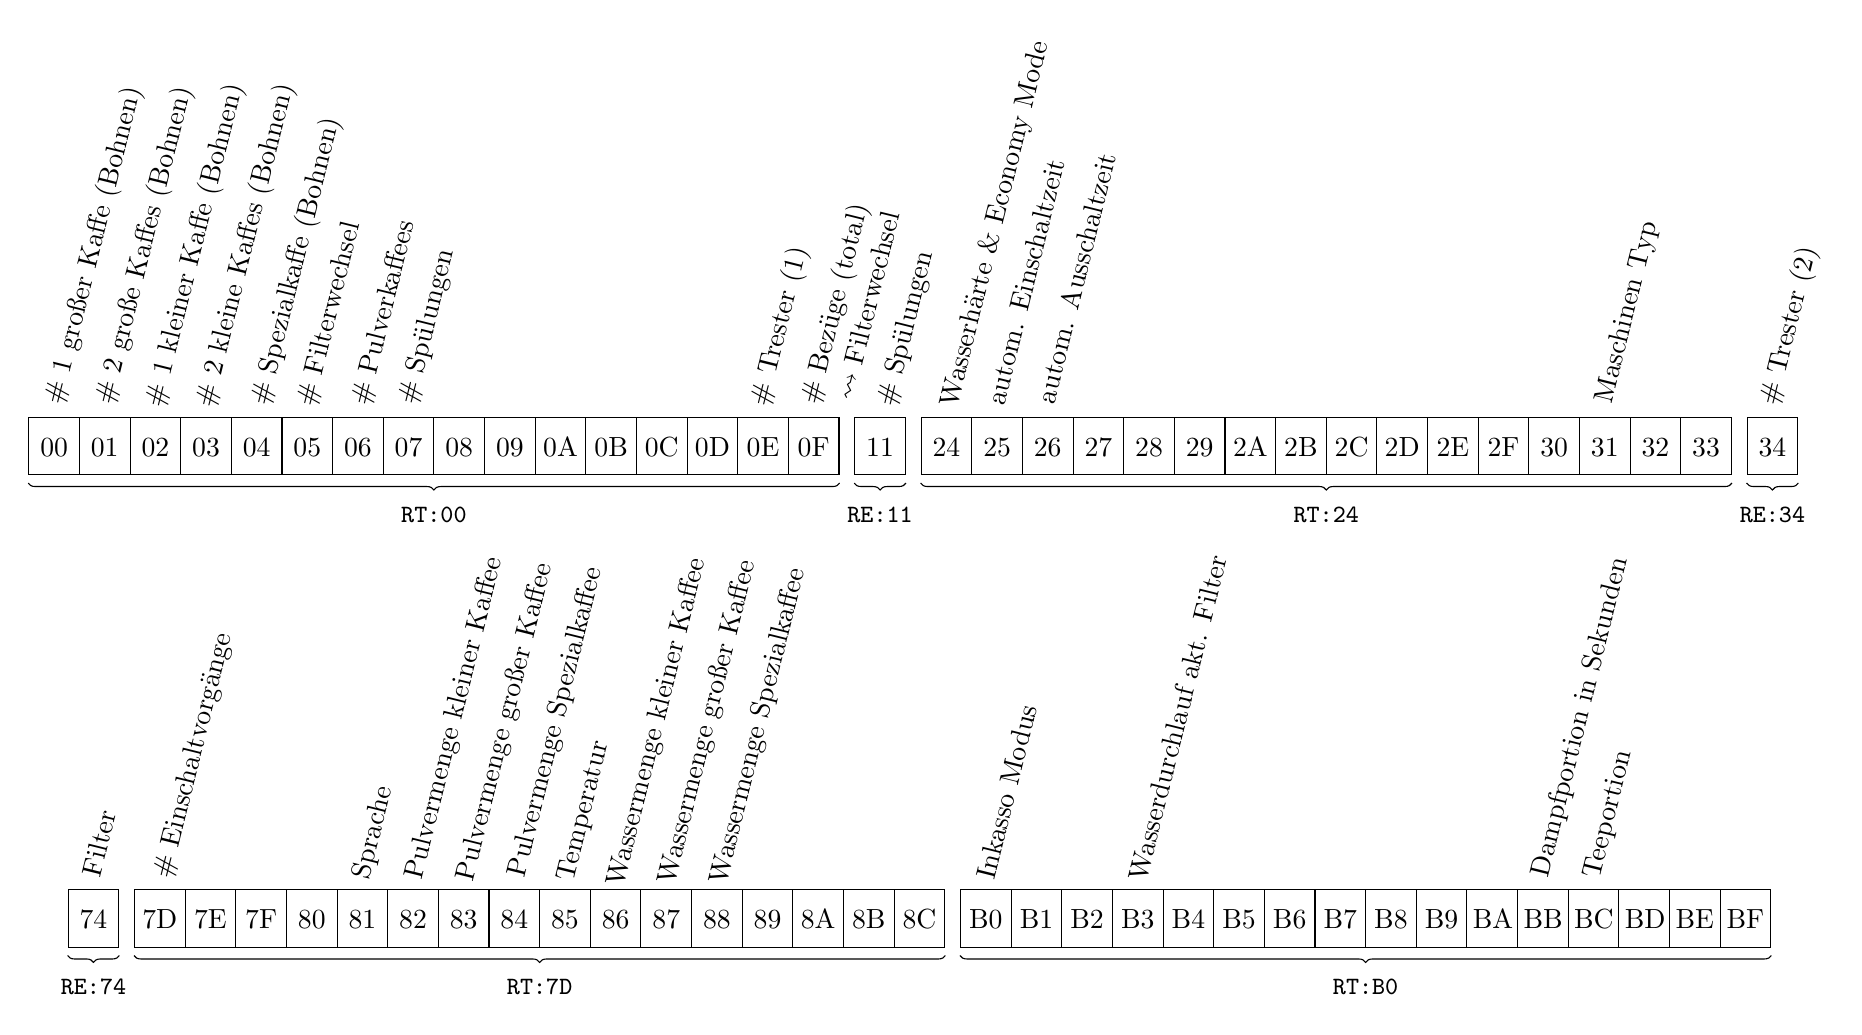
\begin{tikzpicture}[draw, minimum width=1cm, minimum height=0.5cm]
  \matrix[mymat,anchor=west,style={nodes=draw}] at (0,6)
  (Speicher1) {
          |(00)| 00 &
          |(01)| 01 &
          |(02)| 02 &
          |(03)| 03 &
          |(04)| 04 &
          |(05)| 05 &
          |(06)| 06 &
          |(07)| 07 &
          |(08)| 08 &
          |(09)| 09 &
          |(0A)| 0A &
          |(0B)| 0B &
          |(0C)| 0C &
          |(0D)| 0D &
          |(0E)| 0E &
          |(0F)| 0F &
    [2mm]
          |(11)| 11 &
    [2mm]
          |(24)| 24 &
          |(25)| 25 &
          |(26)| 26 &
          |(27)| 27 &
          |(28)| 28 &
          |(29)| 29 &
          |(2A)| 2A &
          |(2B)| 2B &
          |(2C)| 2C &
          |(2D)| 2D &
          |(2E)| 2E &
          |(2F)| 2F &
          |(30)| 30 &
          |(31)| 31 &
          |(32)| 32 &
          |(33)| 33 &
    [2mm]
          |(34)| 34 \\
  };
  
  \matrix[mymat,anchor=west,style={nodes=draw}] at (0.5,0) 
  (Speicher2) {
          |(74)| 74 &
    [2mm]
          |(7D)| 7D &
          |(7E)| 7E &
          |(7F)| 7F &
          |(80)| 80 &
          |(81)| 81 &
          |(82)| 82 &
          |(83)| 83 &
          |(84)| 84 &
          |(85)| 85 &
          |(86)| 86 &
          |(87)| 87 &
          |(88)| 88 &
          |(89)| 89 &
          |(8A)| 8A &
          |(8B)| 8B &
          |(8C)| 8C &
    [2mm]
          |(B0)| B0 &
          |(B1)| B1 &
          |(B2)| B2 &
          |(B3)| B3 &
          |(B4)| B4 &
          |(B5)| B5 &
          |(B6)| B6 &
          |(B7)| B7 &
          |(B8)| B8 &
          |(B9)| B9 &
          |(BA)| BA &
          |(BB)| BB &
          |(BC)| BC &
          |(BD)| BD &
          |(BE)| BE &
          |(BF)| BF \\
  };
  
  \draw[decorate,decoration={brace,mirror,raise=1mm}]
    (00.south west) -- (0F.south east) node [black,midway,yshift=-5mm] {\small\texttt{RT:00}};
  \draw[decorate,decoration={brace,mirror,raise=1mm}]
    (11.south west) -- (11.south east) node [black,midway,yshift=-5mm] {\small\texttt{RE:11}};
  \draw[decorate,decoration={brace,mirror,raise=1mm}]
    (24.south west) -- (33.south east) node [black,midway,yshift=-5mm] {\small\texttt{RT:24}};
  \draw[decorate,decoration={brace,mirror,raise=1mm}]
    (34.south west) -- (34.south east) node [black,midway,yshift=-5mm] {\small\texttt{RE:34}};
  \draw[decorate,decoration={brace,mirror,raise=1mm}]
    (74.south west) -- (74.south east) node [black,midway,yshift=-5mm] {\small\texttt{RE:74}};
  \draw[decorate,decoration={brace,mirror,raise=1mm}]
    (7D.south west) -- (8C.south east) node [black,midway,yshift=-5mm] {\small\texttt{RT:7D}};
  \draw[decorate,decoration={brace,mirror,raise=1mm}]
    (B0.south west) -- (BF.south east) node [black,midway,yshift=-5mm] {\small\texttt{RT:B0}};
    
  \node [above=22mm of 00,rotate=76,yshift=-8mm,xshift=1mm] {\# 1 großer Kaffe (Bohnen)};
  \node [above=22mm of 01,rotate=76,yshift=-8mm,xshift=1mm] {\# 2 große Kaffes (Bohnen)};
  \node [above=22mm of 02,rotate=76,yshift=-8mm,xshift=1mm] {\# 1 kleiner Kaffe (Bohnen)};
  \node [above=22mm of 03,rotate=76,yshift=-8mm,xshift=1mm] {\# 2 kleine Kaffes (Bohnen)};
  \node [above=20mm of 04,rotate=76,yshift=-8mm,xshift=1mm] {\# Spezialkaffe (Bohnen)};
  \node [above=12.7mm of 05,rotate=76,yshift=-5.5mm,xshift=1mm] {\# Filterwechsel};
  \node [above=13mm of 06,rotate=76,yshift=-6mm,xshift=1mm] {\# Pulverkaffees};
  \node [above=11mm of 07,rotate=76,yshift=-5mm,xshift=1mm] {\# Spülungen};
  \node [above=11mm of 0E,rotate=76,yshift=-5mm,xshift=1mm] {\# Trester (1)};
  \node [above=14mm of 0F,rotate=76,yshift=-9mm,xshift=1mm,align=right] {\# Bezüge (total)\\$\leadsto$ Filterwechsel};
  \node [above=11mm of 11,rotate=76,yshift=-6mm,xshift=1mm] {\# Spülungen};
  \node [above=25mm of 24,rotate=76,yshift=-9mm,xshift=1mm] {Wasserhärte \& Economy Mode};
  \node [above=17mm of 25,rotate=76,yshift=-6mm,xshift=1mm] {autom. Einschaltzeit};
  \node [above=17.5mm of 26,rotate=76,yshift=-6mm,xshift=1mm] {autom. Ausschaltzeit};
  \node [above=13mm of 31,rotate=76,yshift=-5.5mm,xshift=1mm] {Maschinen Typ};
  \node [above=11mm of 34,rotate=76,yshift=-5mm,xshift=1mm] {\# Trester (2)};
  \node [above=5mm of 74,rotate=76,yshift=-3mm,xshift=1mm] {Filter};
  \node [above=17mm of 7D,rotate=76,yshift=-7mm,xshift=1mm] {\# Einschaltvorgänge};
  \node [above=6.5mm of 81,rotate=76,yshift=-4mm,xshift=1mm] {Sprache};
  \node [above=22mm of 82,rotate=76,yshift=-8mm,xshift=1mm] {Pulvermenge kleiner Kaffee};
  \node [above=21.5mm of 83,rotate=76,yshift=-8mm,xshift=1mm] {Pulvermenge großer Kaffee};
  \node [above=21.5mm of 84,rotate=76,yshift=-8mm,xshift=1mm] {Pulvermenge Spezialkaffee};
  \node [above=9.5mm of 85,rotate=76,yshift=-5mm,xshift=1mm] {Temperatur};
  \node [above=21.5mm of 86,rotate=76,yshift=-8mm,xshift=1mm] {Wassermenge kleiner Kaffee};
  \node [above=21.5mm of 87,rotate=76,yshift=-8mm,xshift=1mm] {Wassermenge großer Kaffee};
  \node [above=21mm of 88,rotate=76,yshift=-8mm,xshift=1mm] {Wassermenge Spezialkaffee};
  \node [above=12mm of B0,rotate=76,yshift=-5mm,xshift=1mm] {Inkasso Modus};
  \node [above=22mm of B3,rotate=76,yshift=-7.5mm,xshift=1mm] {Wasserdurchlauf akt. Filter};
  \node [above=22mm of BB,rotate=76,yshift=-7.5mm,xshift=1mm] {Dampfportion in Sekunden};
  \node [above=9mm of BC,rotate=76,yshift=-4.5mm,xshift=1mm] {Teeportion};
\end{tikzpicture}



\end{document}
